\chapter{Operation of the \abbrROV} \label{app:operation}
This Chapter describes normal operation of the \abbrROV, how to implement new controllers and some tips for troubleshooting.

\section{Wiring} \label{sec_wiring}
\todo[inline]{Write about how wire the \abbrROV} 
%%%%%%%%%%%%%%%%%%%%%%%%%%%%%%%%%%%%%%%%%%%%%%%%
\section{Start up of the \abbrROV}
For starting the \abbrROV connect all cables according to \Sectionref{sec:wiring}.
\begin{itemize}
	\item Make sure that the battery is tightly fastened and is fully charged. 
	\item Slide the cradle gently into the \abbrROV tube. 
	\item If needed apply some silicone grease to the O-rings of the end cap. Then slide the end cap into the \abbrROV tube.
	\item Insert the vent bolt in to the vent nut on the end cap.
	\item Insert the cat 6 cable to the workstation.
 \end{itemize} 
Navigate to the catkin\_ws folder on the workstation and run the start script in a terminal for the \abbrROV
\begin{lstlisting}
 ./startrov.sh
\end{lstlisting}
Then in a new terminal navigate to the catkin\_ws folder and run the workstation script
\begin{lstlisting}
 ./startworkstation.sh
\end{lstlisting} 
%%%%%%%%%%%%%%%%%%%%%%%%%%%%%%%%%%%%%%%%%%%%%%%%
\section{Operating the ROV}

\subsection{Modes and controllers}

\subsubsection{Manual mode}

\subsection{Logging data}\label{sec:logging}
For logging data rqt-bag or the supplied script can be used. In rqt on the workstation start rqt-bag by Plugins $\rightarrow$ Logging $\rightarrow$ Bag. Start the recording of data by pressing the red circle. A menu of available topics is showed, select the topics that you want to record. Then give the logfile a name in the pop-up.
To stop recording data press the red circle and close Bag by Running $\rightarrow$ Close:Bag. For using the logging scripts use 
\begin{lstlisting}
./test.sh
\end{lstlisting}
and follow the instructions.

\subsection{Sending test signals}
For sending telegraph signals to the \abbrROV the logging script in \Sectionref{sec:logging} can be used or dynamic reconfigure can be used. Dynamic reconfigure can be used from the command line or rqt. In rqt start dynamic reconfigure by Plugins $\rightarrow$ Configuration $\rightarrow$ Dynamic Reconfigure. When the dynamic reconfigure box is shown choose matlab\_controller then check telegraph\_signals. In the submenu choose the scaling and switch factor for each thruster. Then the wanted thrusters has to be enabled/disabled by checking/unchecking the option \textit{enable_thrusteri}. To enable tests change the test signal from off $\rightarrow$ on.    

\subsection{Displaying the continuous plots}
Displaying plots in rqt is enabled by Plugins $\rightarrow$ Visualization $\rightarrow$ Plot. In the plot plugin, data can be plotted by choosing topics in the topic field this is shown in \Figureref{fig:contplot}. The active topics can be seen in the command line by running 
\begin{lstlisting}
rostopic list
\end{lstlisting}
\begin{figure}
\centering
\begin{tikzpicture}
    \node[anchor=south west,inner sep=0] (image) at (0,0) {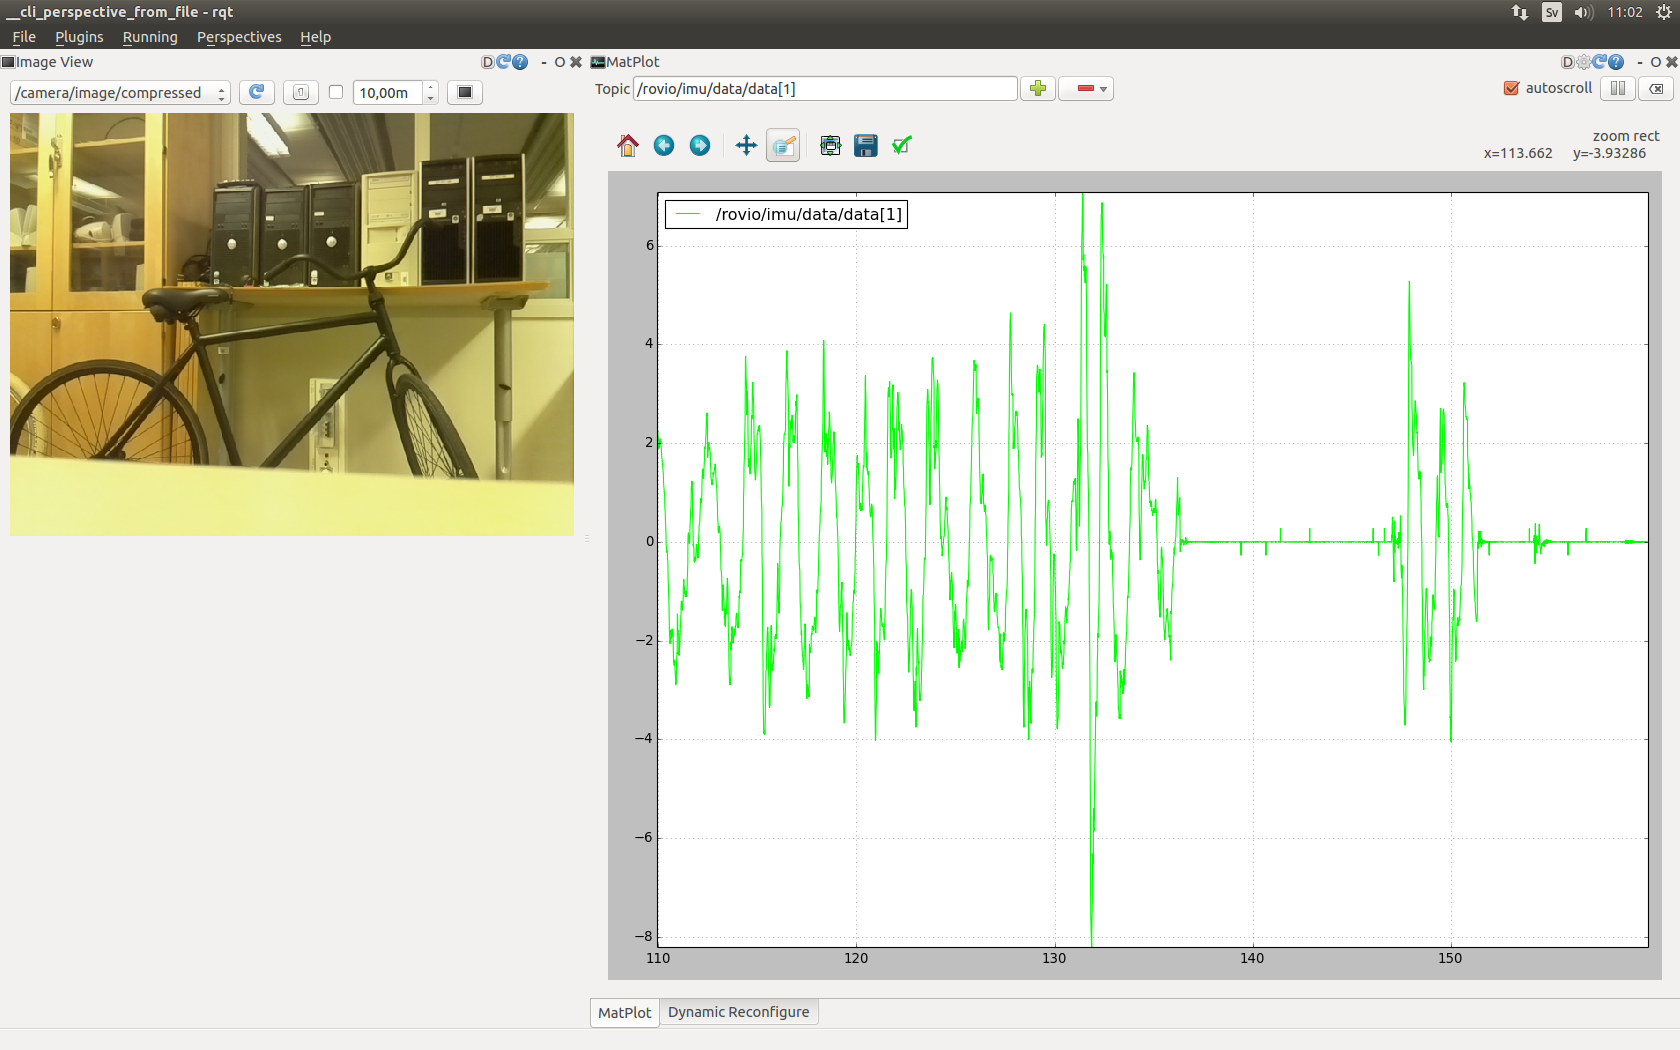
\includegraphics[trim={0cm 0cm 0cm 0.8cm},clip,width=0.9\textwidth]{contplot}};
    \begin{scope}[x={(image.south east)},y={(image.north west)}]
        \draw[red,ultra thick,rounded corners] (0.35,0.91) rectangle (0.67,0.96);
    \end{scope}
\end{tikzpicture}
\caption{The topic field where the specification of what data should be plotted is circled in red. The green plus adds data to be plotted and the red minus removes data from the graph.}
\label{fig:contplot}
\end{figure}

For multiarray messages an extra \textit{\textbackslash data} field has to be added to the topic. Data is then accessed by indexing with hard brackets. 
\begin{example}
Plot the data with index 1 in the multiarray message on topics \textit{/rovio/imu/data}. Type /rovio/imu/data/data[1] in the into the topic field and press the green plus.  
\end{example}

\subsection{\abbrLED lights on the HKPilot}
There are several different \abbrLED lights on the HKPilot Mega 2.7, \Tableref{tab:ledStatus} summaries some of \abbrLED statuses
 \begin{table}[tbp]
  \centering
  \caption{\label{tab:ledStatus}%
    Some of the \abbrLED statues used by the HKPilot Mega 2.7.}
  \begin{tabular}{l p{0.7\linewidth}}
    \toprule%
    \textbf{Light}  & \textbf{Description} \\
    \otoprule%
    Red 				& The HKPilot is setting up sensors and a connection to \abbrROS. The red light won't turn off until the connection to \abbrROS has been established.\\
    \midrule
    Pulsating blue 	& Pulsating blue light indicate that the HKPilot has connection with the workstation.\\
    \midrule
    Yellow 			& Shows that the \abbrROV is disarmed. \\
    \bottomrule%
  \end{tabular}
\end{table}

%%%%%%%%%%%%%%%%%%%%%%%%%%%%%%%%%%%%%%%%%%%%%%%%
\section{New Parameter Estimation and New Controllers}

\subsection{New Parameter Estimation}

\subsection{New Controllers}
To implement a new controller open the Simulink file Controller.slx. Construct the controller in a suitable location. Then expand the switch that chooses what controller that is used, see \Figureref{fig:controller_simulink}. Connect the new controller to the switch to enable that the controller can be chosen from dynamic reconfigure when operating the \abbrROV.

\begin{figure}
\centering
\begin{tikzpicture}
    \node[anchor=south west,inner sep=0] (image) at (0,0) {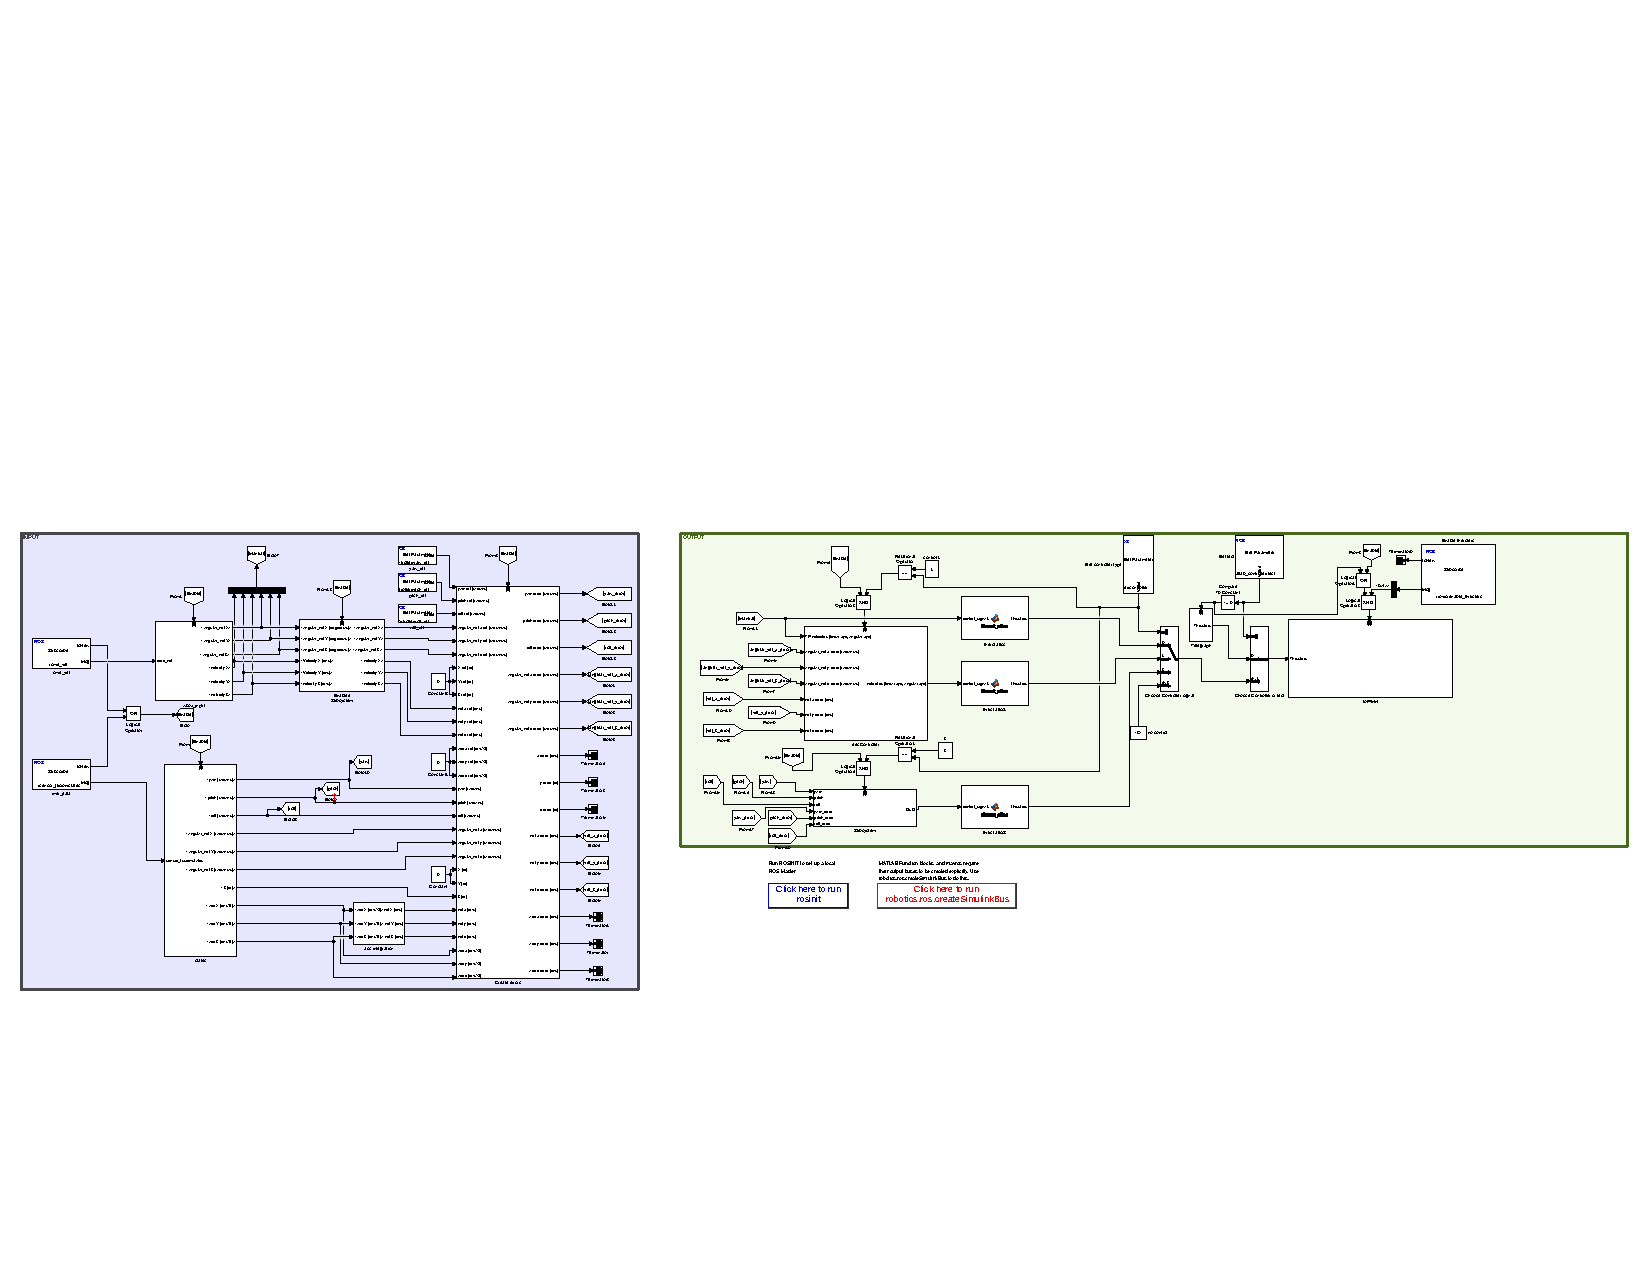
\includegraphics[trim={18cm 7cm 2.5cm 9cm},clip,width=0.9\textwidth]{Controller}};
    \begin{scope}[x={(image.south east)},y={(image.north west)}]
        \draw[red,ultra thick,rounded corners] (0.20,0.48) rectangle (0.28,0.75);
    \end{scope}
\end{tikzpicture}
    \caption{When implementing new controllers in the control node the red marked switch has to be expanded. The new controller ought to be connected to the new connector for enabling the usage of the controller.}
    \label{fig:controller_simulink}
\end{figure}

\subsection{Code Generation of the Controller Node}


%%%%%%%%%%%%%%%%%%%%%%%%%%%%%%%%%%%%%%%%%%%%%%%%
\section{Known issues and troubleshooting}
This sections brings up some of the known issues and how to solve them. Some general debugging and troubleshooting is also brought up.

\subsection{Calibration of Sensors}
If drift or bias is noted in the sensor fusion or in the raw sensor reading it could be due to bad calibration of the sensors.
Calibration of the gyroscope is done by
\begin{lstlisting}
rostopic pub --once /rovio/gyro/calibrate_offsets std_msgs/Bool true
\end{lstlisting}
The calibration of the accelerometer is done by running
\begin{lstlisting}
rostopic pub --once /rovio/accelerometer/calibrate_offsets std_msgs/Bool true
\end{lstlisting}
and following the instructions that shows up.
Calibration of the magnetometer is done by the command
\begin{lstlisting}
rostopic pub --once /rovio/magnetometer/calibrate_offsets std_msgs/Bool true
\end{lstlisting}
and following the commands that shows up.
For setting the magnetic field in the sensor fusion run 
\begin{lstlisting}
./calibratemag.sh
\end{lstlisting}

\subsection{\abbrROS Debugging}
Debugging \abbrROS nodes can be done by listening on \abbrROS messages. This is done by 
\begin{lstlisting}
rostopic echo /example/topic
\end{lstlisting}
In the nodes several different log messages can be generated for example by \textit{ROS\_INFO} and \textit{ROS\_DEBUG}.

\subsection{Check Ethernet Connection}
It is assumed that the setup from \Appref{app:dependencies} is done. To check the Ethernet connection from the \abbrROV to the workstation or the other way around do
\begin{lstlisting}
#From the ROV to the workstation
ping -c 10 10.0.0.10 
#From the workstation to the ROV
ping -c 10 10.0.0.20
\end{lstlisting}
If the connection is good the output ought to be something like 64 bytes received from 10.0.0.10... Otherwise the connection has to be checked. Check that the Ethernet cable is connected and that both the \abbrROV and workstation is powered on. Check that both the workstation and the \abbrROV has the correct \abbrIP by the command
\begin{lstlisting}
ifconfig
\end{lstlisting}
The output at eth0 ought to contain the correct \abbrIP. Otherwise the setup from the \Appref{app:dependencies} has to revisited.

\subsection{One or Several Thrusters Are Unresponsive}\label{subsec:unresponsive}
To check for unresponsive thrusters run the following commands 
\begin{lstlisting}
rostopic pub --once /rovio/thrusters_enable std_msgs/Bool true
./thrusterTest.sh
\end{lstlisting}
The thruster test will run the thrusters at a minimal torque in incremental order. If the one or several thrusters are unresponsive check that the thrusters are connected according to \Sectionref{sec:wiring}. If all thrusters are unresponsive check that the HKPilot Mega 2.7 and the Raspberry has power and connected to each other. Note that if the \abbrROV is disarmed no control signals will be sent to the thrusters.

\subsection{Checking and changing rotation of thrusters}
The rotation of thrusters are important due to the moments they create. Thus are two thruster pairs counter-rotating. For checking the rotation of the thrusters the script mentioned in \Subsectionref{subsec:unresponsive} can be run. \Figureref{fig:thrusterRotation12} - \Figureref{fig:thrusterRotation6} shows how the different thrusters should rotate when supplied with a positive control signal. If one or more thrusters are rotating in the wrong direction, change the order the corresponding thruster cables are connected. 

\begin{figure}
\centering
\begin{tikzpicture}        zb = -0.05/2;
        Kp = -0.5/2;
        Kp_dot = -1/10;
        Kp_abs_p = -1/10;
        Mq = -0.5;
        Mq_dot = -1/10;
        Mq_abs_q = -1/10;
        Nr = -0.5;
        Nr_dot = -1/10;
        Nr_abs_r = -1/10;
        Ix = 0.5;
        Iy = 0.5;
        Iz = 0.5;
        Ix_Kp_dot = Ix - Kp_dot;
        Iy_Mq_dot = Iy - Mq_dot;
        Iz_Nr_dot = Iz - Nr_dot;

    \node[anchor=south west,inner sep=0] (image) at (0,0) {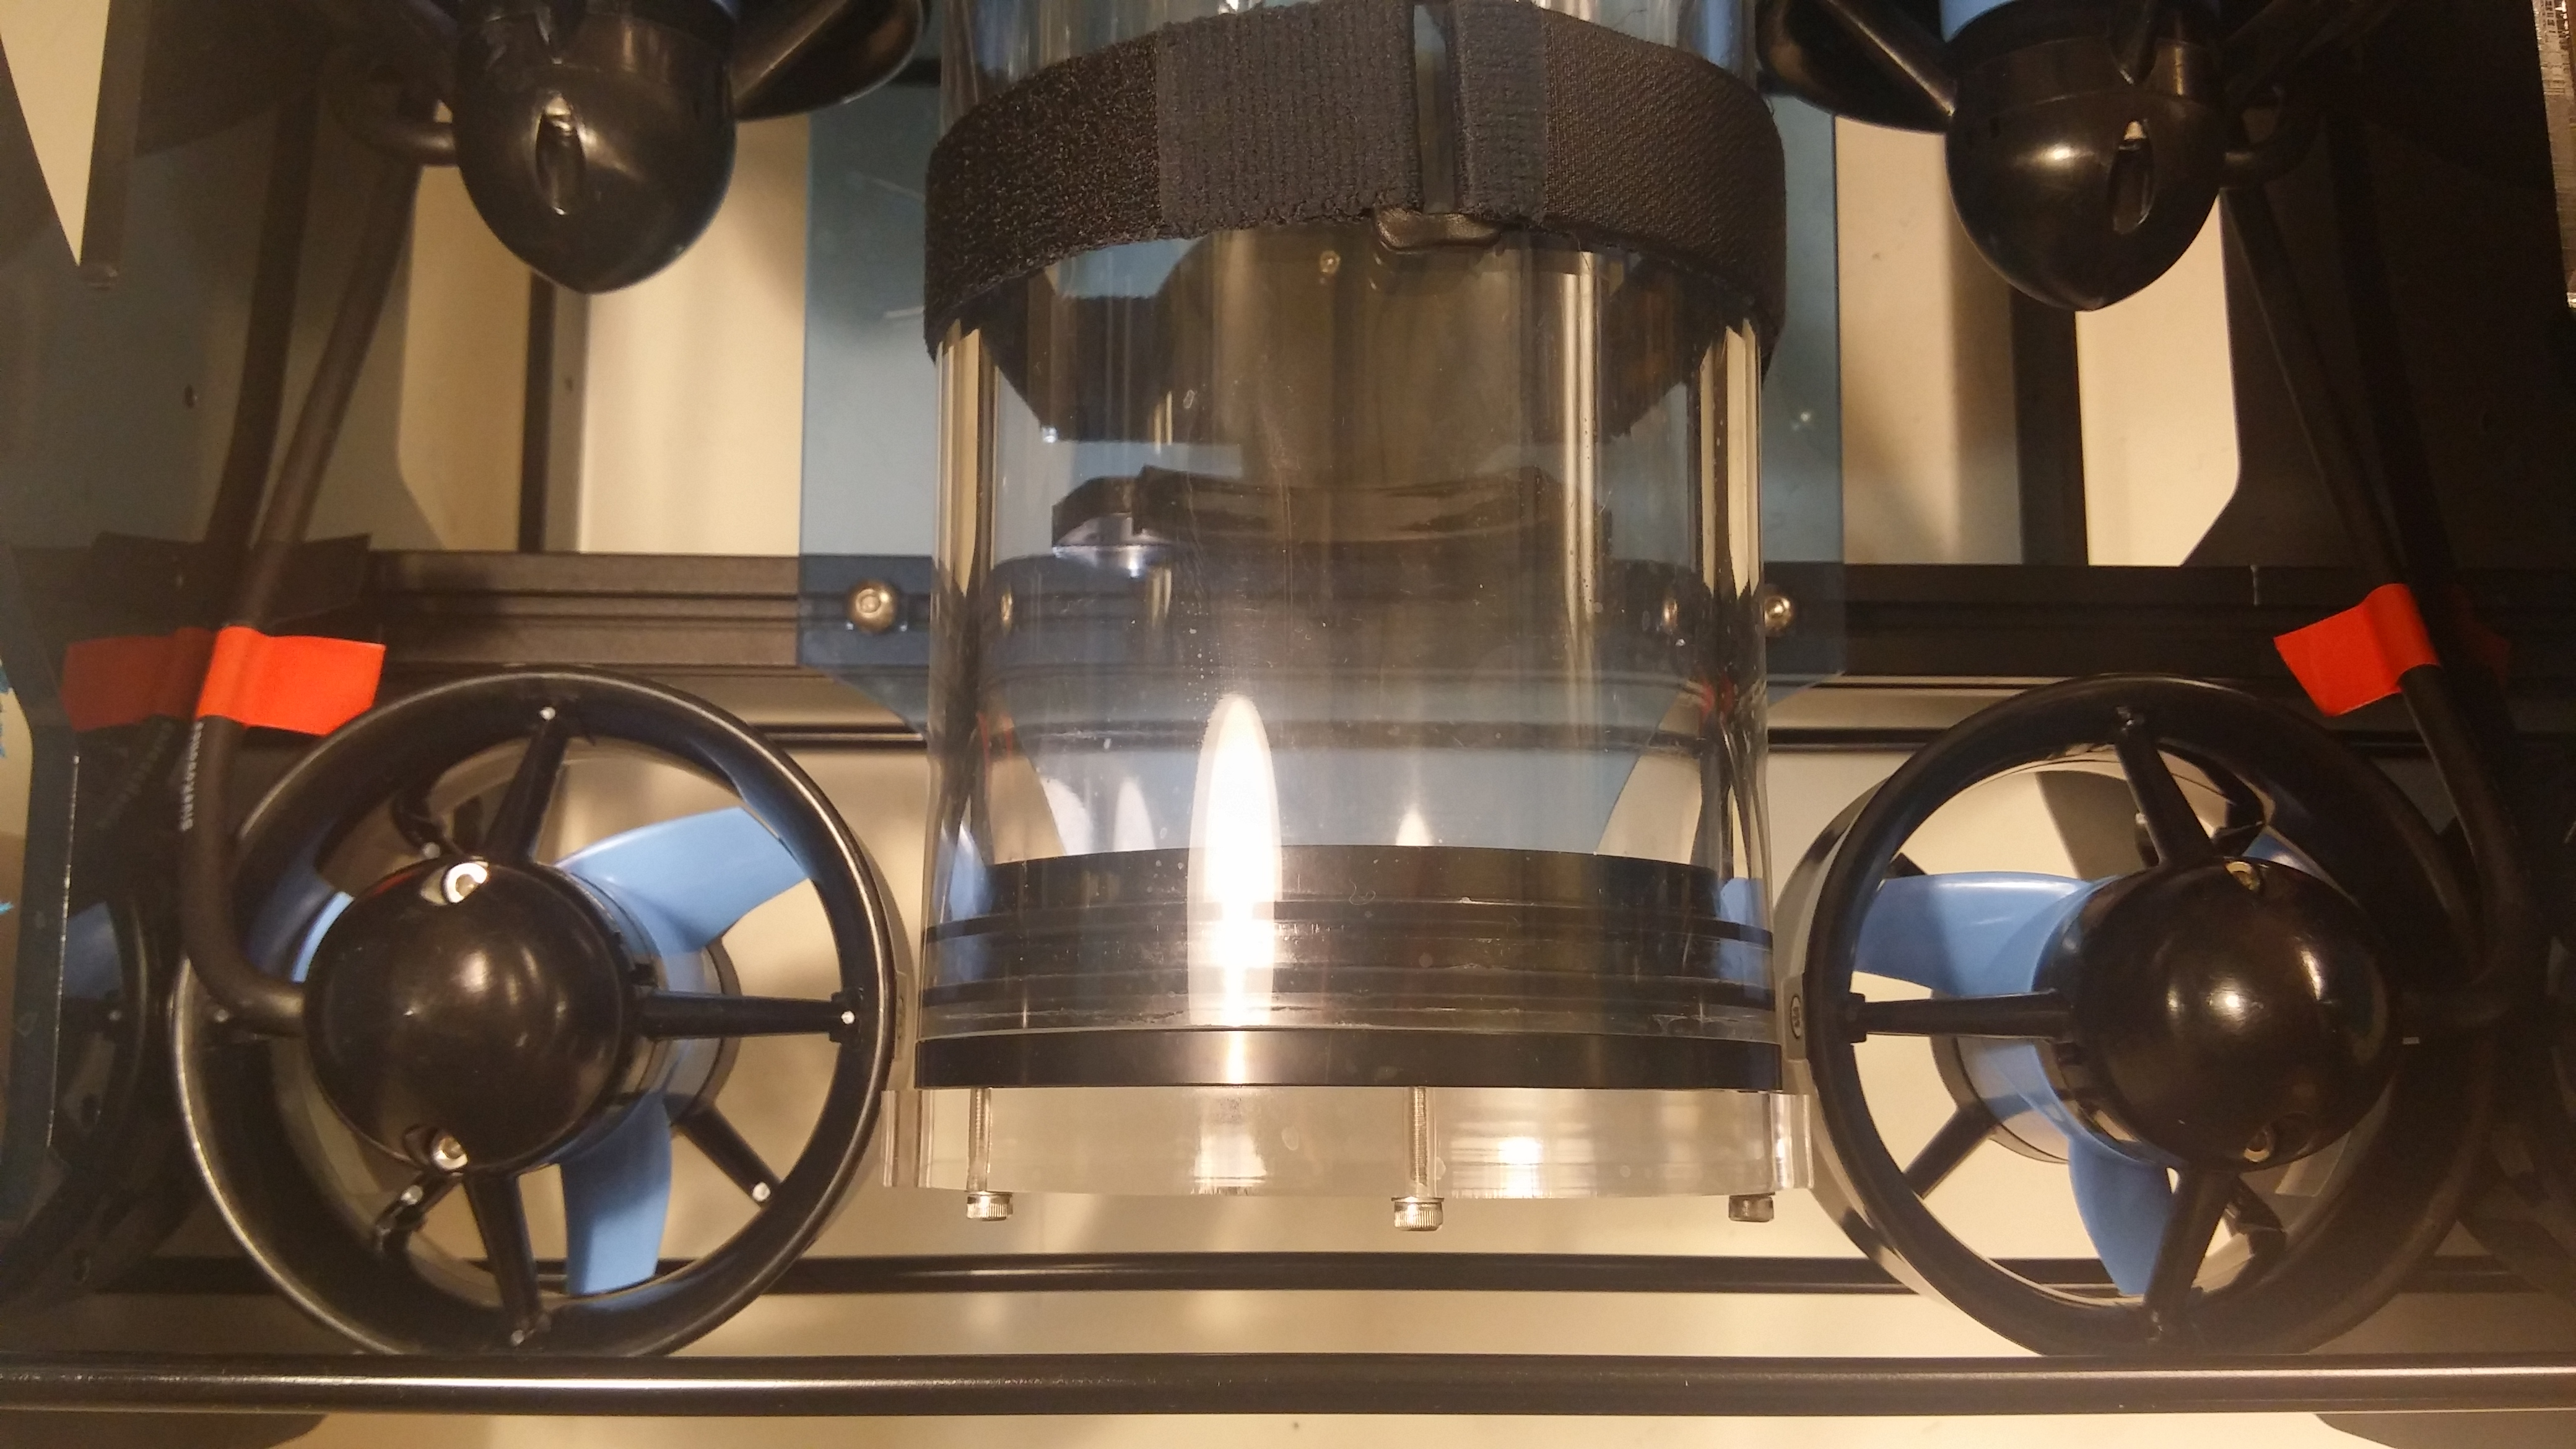
\includegraphics[trim={0cm 0cm 0cm 0cm},clip,width=0.9\textwidth]{thrusterRotation12}};
    \begin{scope}[x={(image.south east)},y={(image.north west)}]
        \draw[->,red,ultra thick,rounded corners] (0.28,0.205) arc (-30:30:0.2);
        \draw[->,red,ultra thick,rounded corners] (0.78,0.205) arc (210:150:0.2);
    \end{scope}
\end{tikzpicture}
    \caption{The arrows indicate the rotational direction of thruster 1 and thruster 2 when supplying a positive control signal.}
    \label{fig:thrusterRotation12}
\end{figure}

\begin{figure}
\centering
\begin{tikzpicture}
    \node[anchor=south west,inner sep=0] (image) at (0,0) {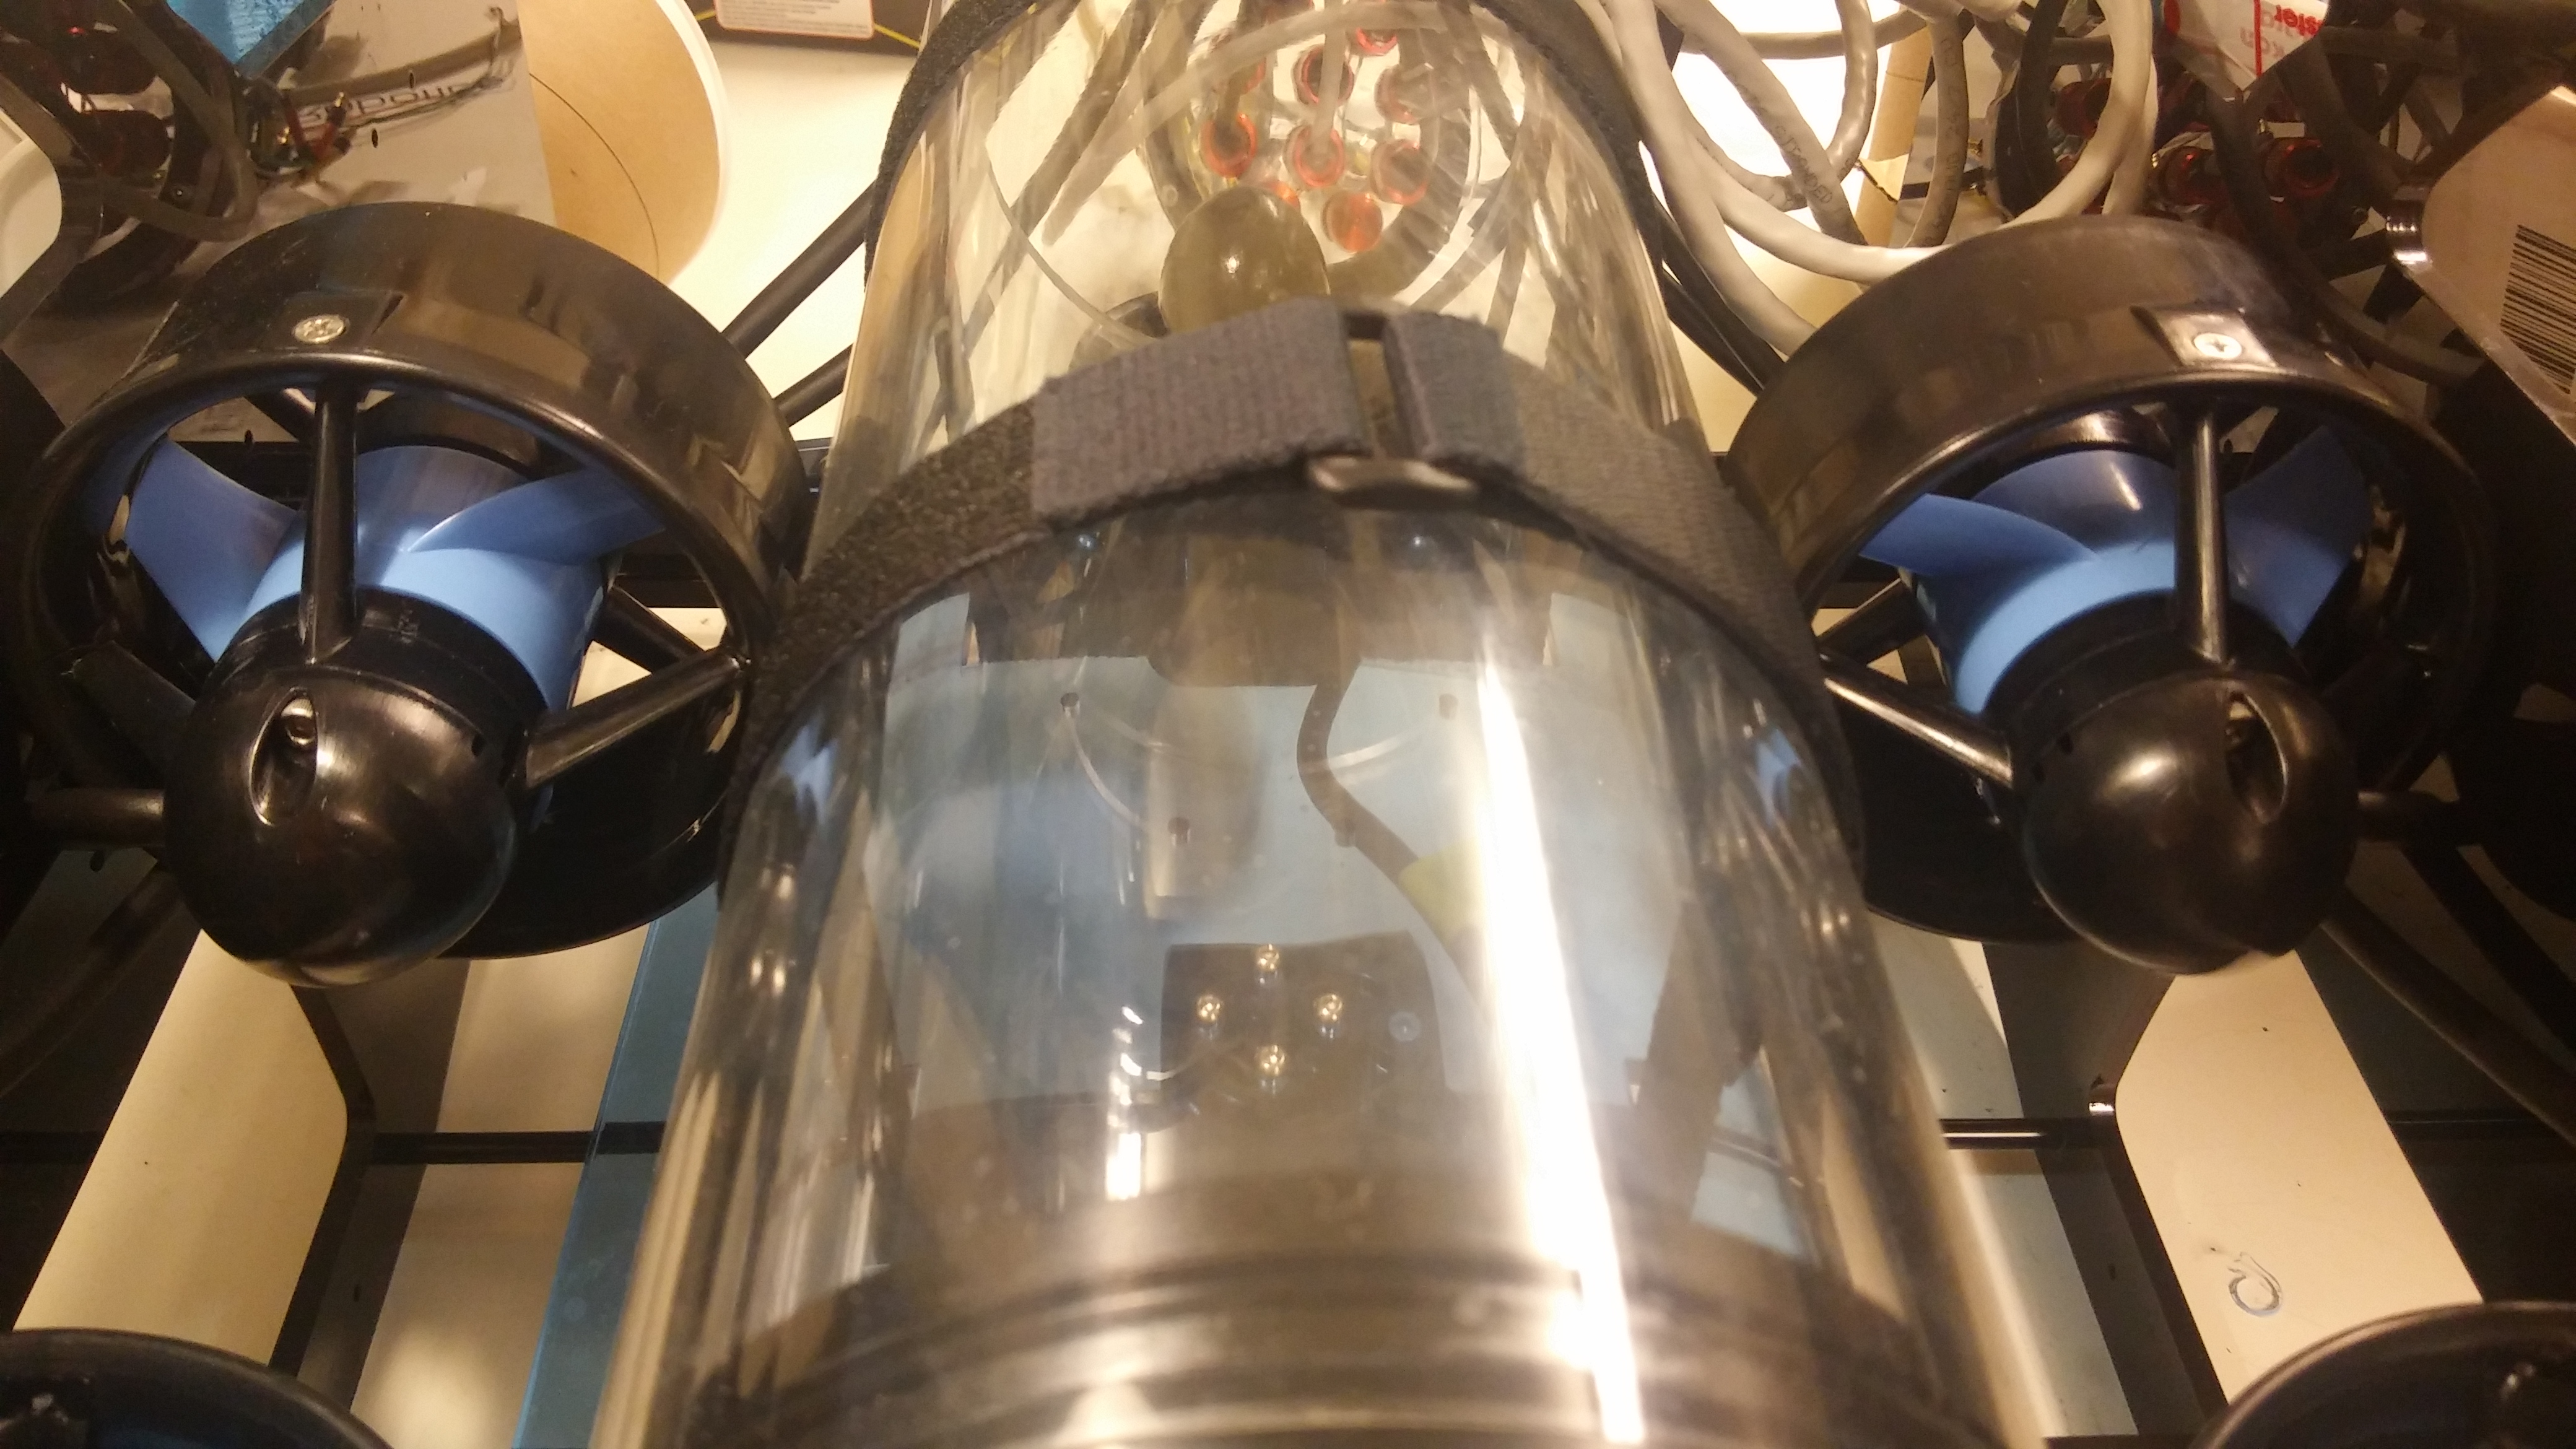
\includegraphics[trim={0cm 0cm 0cm 4cm},clip,width=0.9\textwidth]{thrusterRotation34}};
    \begin{scope}[x={(image.south east)},y={(image.north west)}]
        \draw[->,red,ultra thick,rounded corners] (0.24,0.405) arc (-30:30:0.2);
        \draw[->,red,ultra thick,rounded corners] (0.74,0.405) arc (210:150:0.2);
    \end{scope}
\end{tikzpicture}
    \caption{The arrows indicate the rotational direction of thruster 3 and thruster 4 when supplying a positive control signal.}
    \label{fig:thrusterRotation34}
\end{figure}

\begin{figure}
\centering
\begin{tikzpicture}
    \node[anchor=south west,inner sep=0] (image) at (0,0) {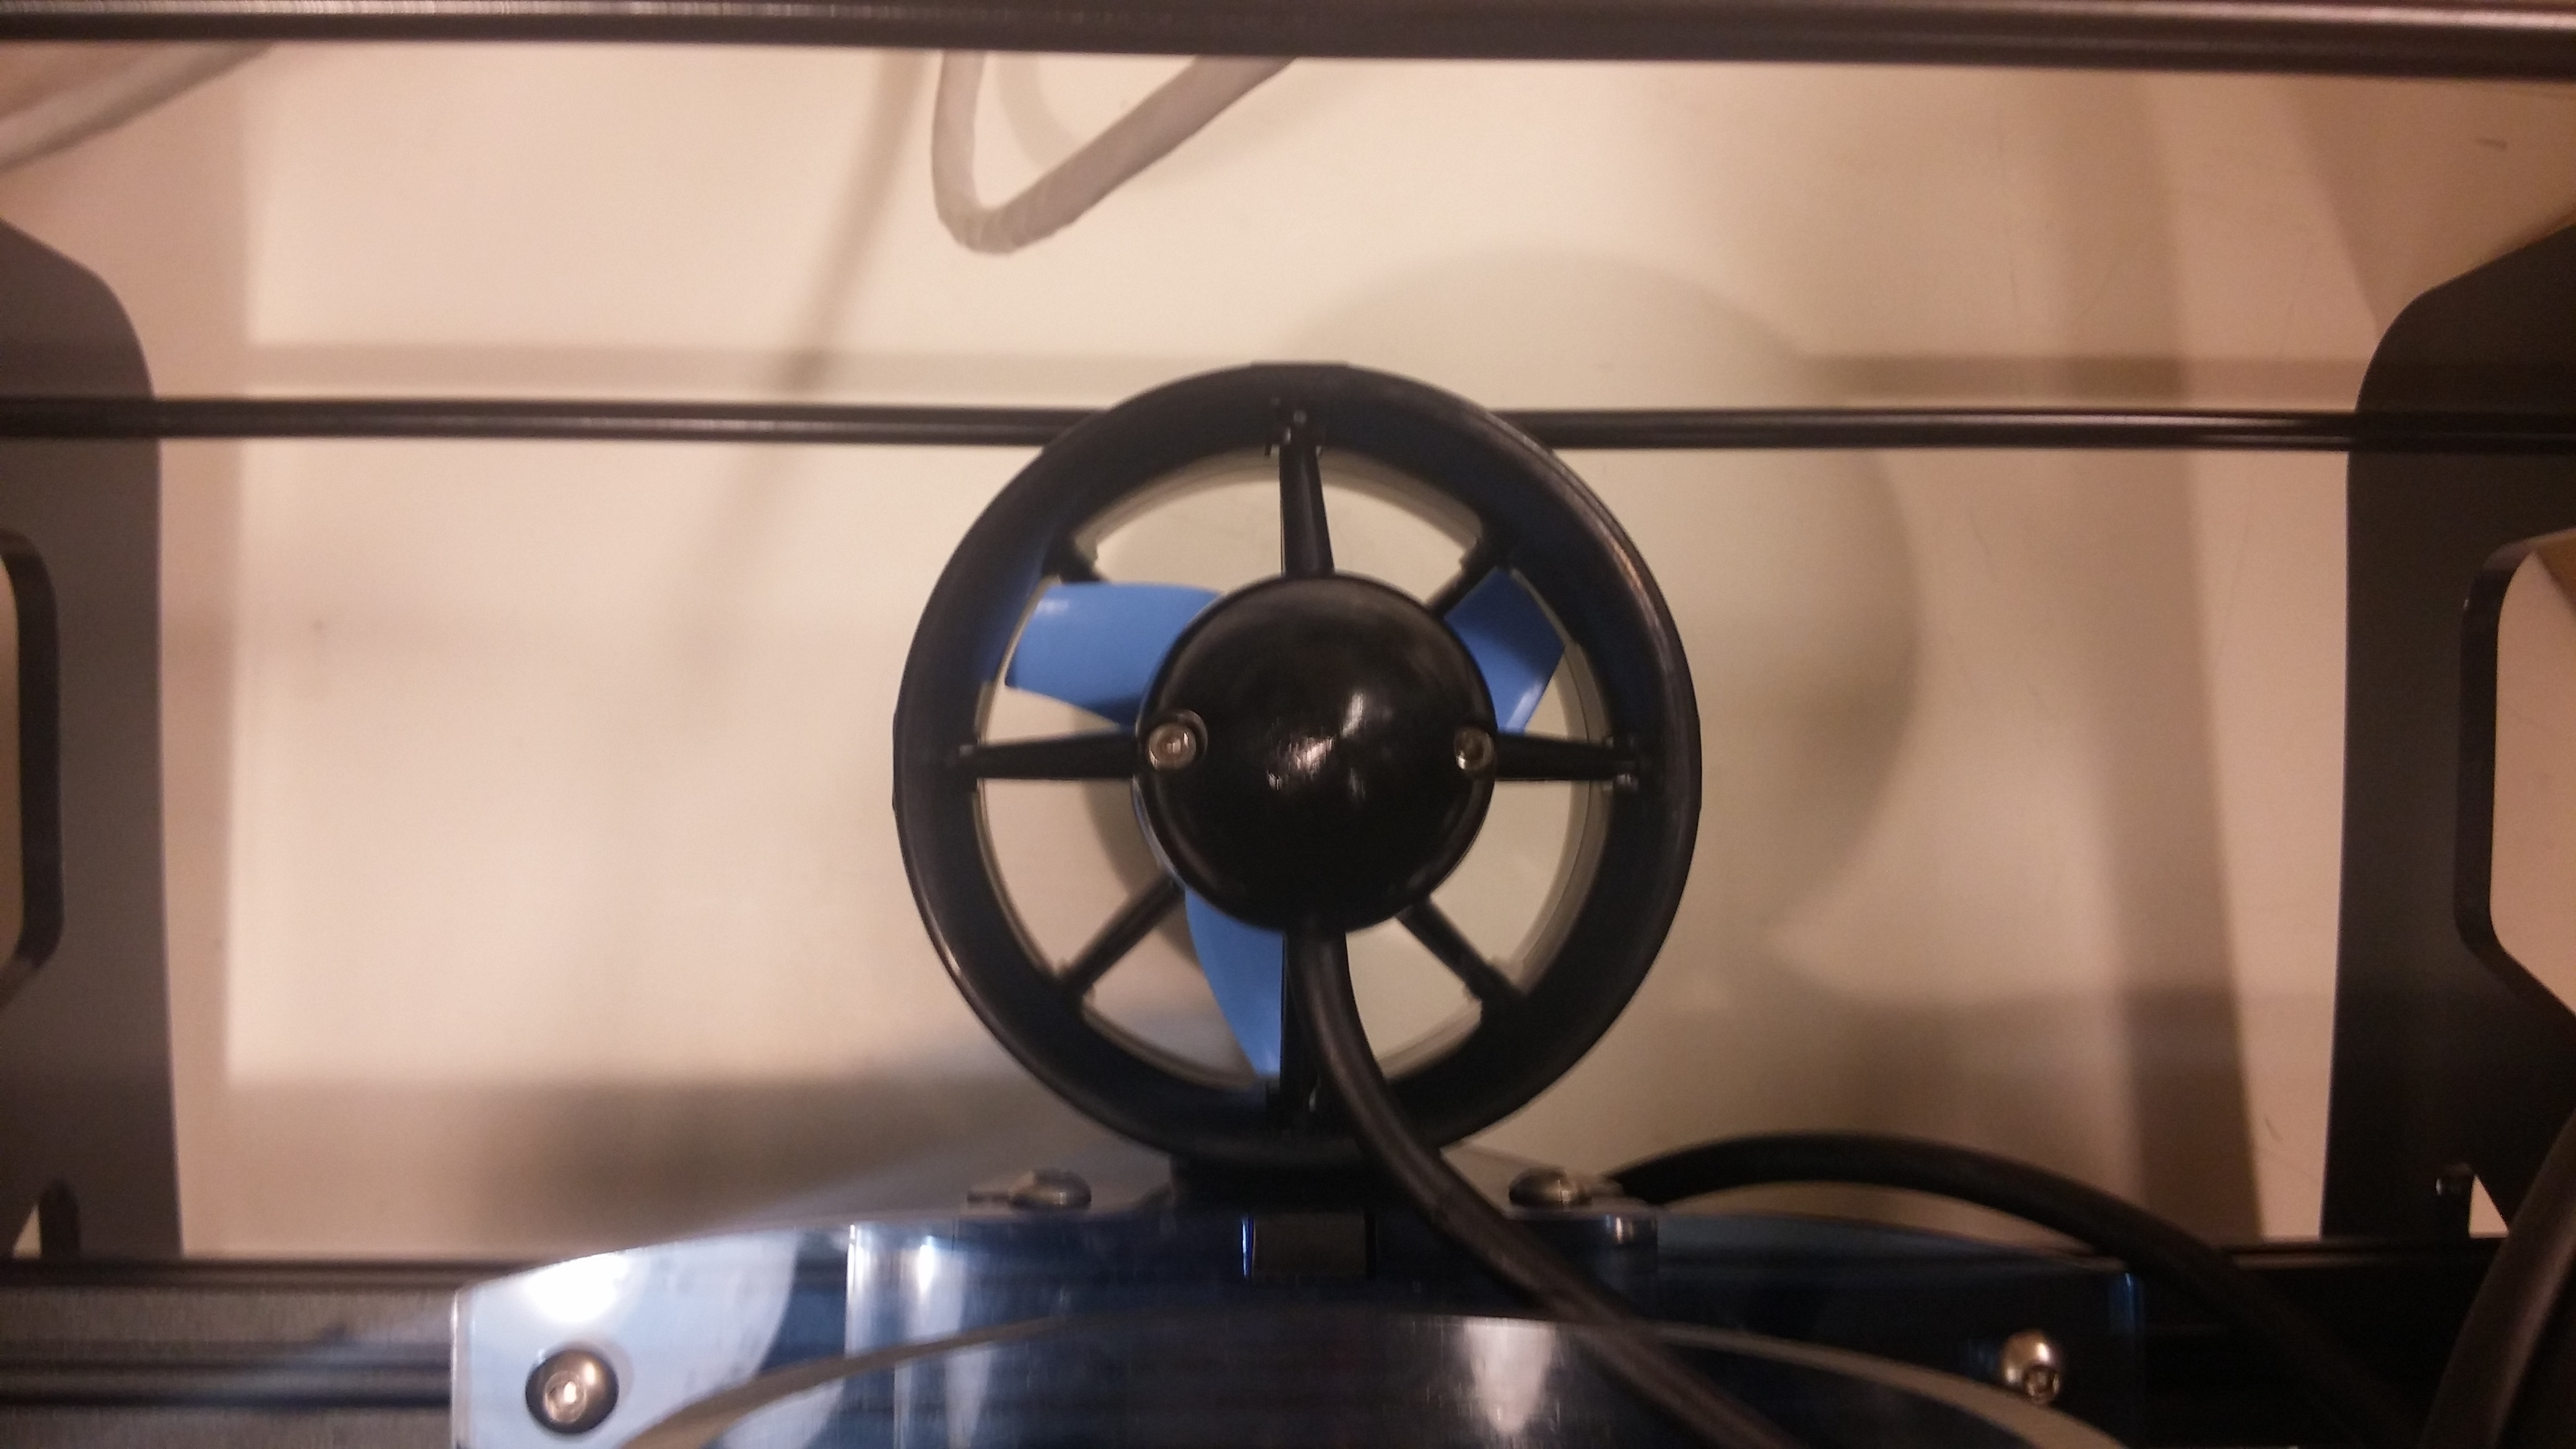
\includegraphics[trim={0cm 0cm 0cm 14cm},clip,width=0.9\textwidth]{thrusterRotation5}};
    \begin{scope}[x={(image.south east)},y={(image.north west)}]
        \draw[->,red,ultra thick,rounded corners] (0.44,0.445) arc (210:150:0.2);
    \end{scope}
\end{tikzpicture}
    \caption{The arrows indicate the rotational direction of thruster 5 when supplying a positive control signal.}
    \label{fig:thrusterRotation5}
\end{figure}

\begin{figure}
\centering
\begin{tikzpicture}
    \node[anchor=south west,inner sep=0] (image) at (0,0) {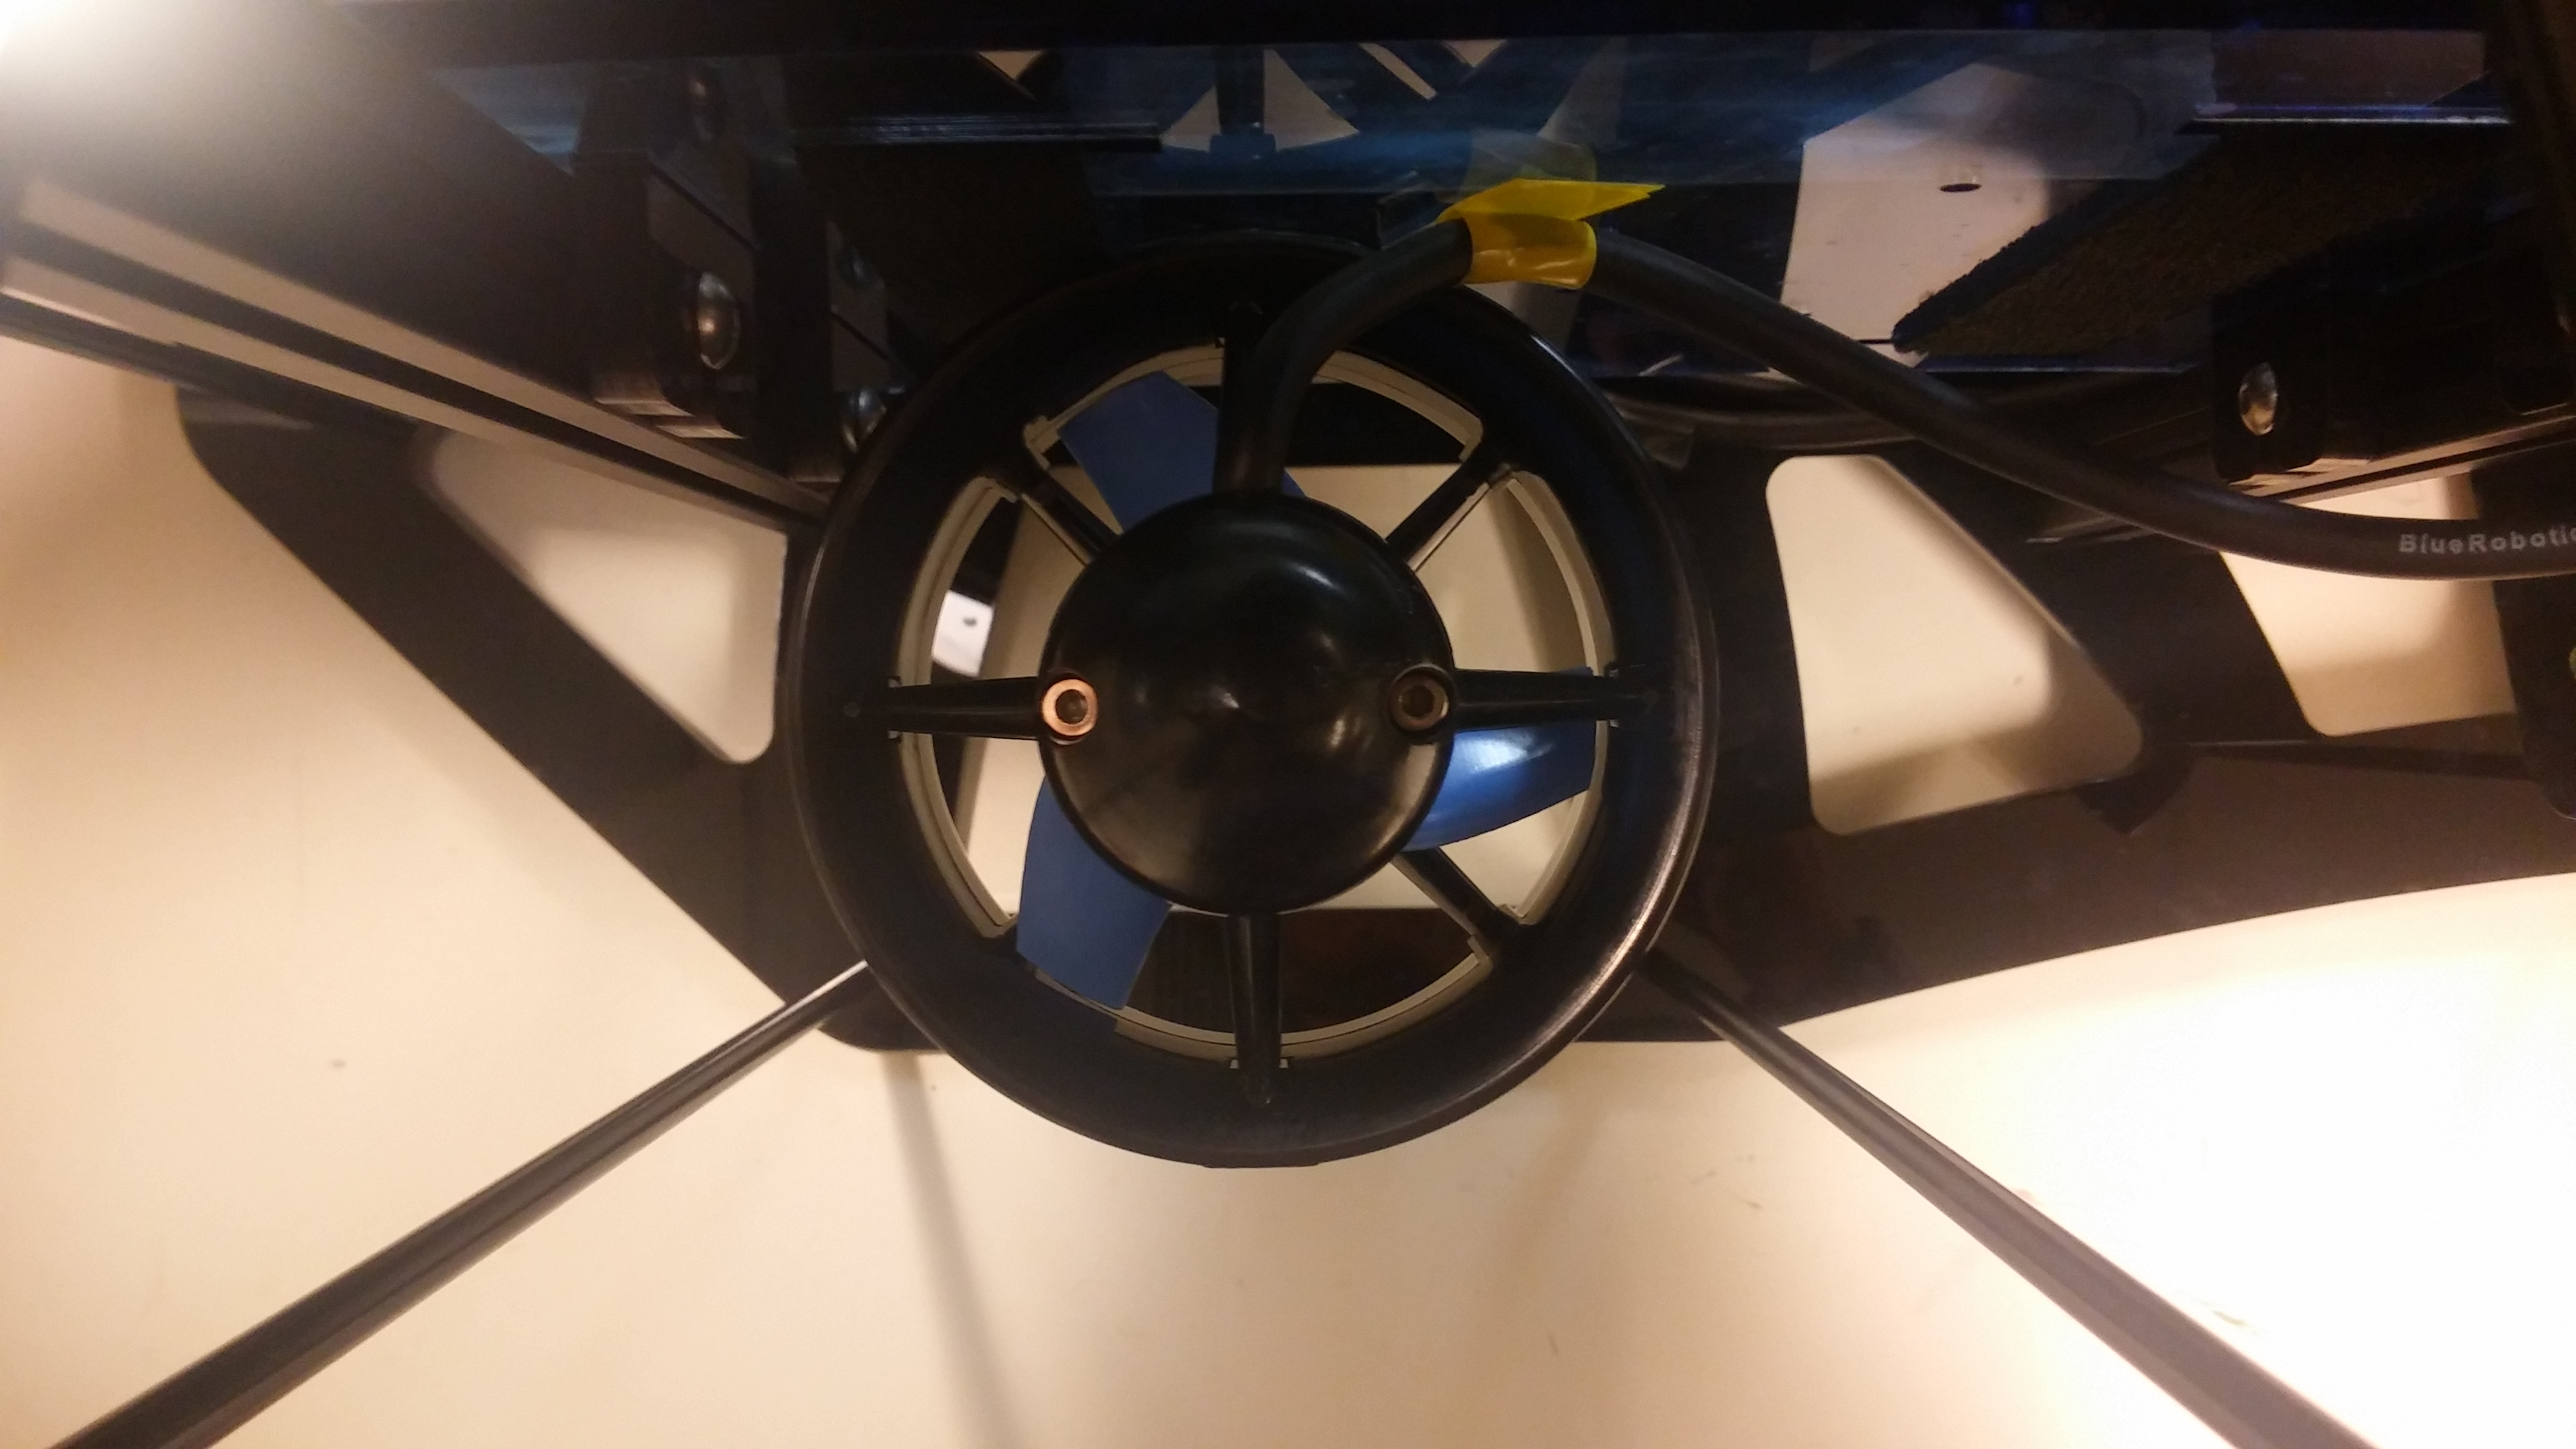
\includegraphics[trim={0cm 0cm 0cm 9cm},clip,width=0.9\textwidth]{thrusterRotation6}};
    \begin{scope}[x={(image.south east)},y={(image.north west)}]
        \draw[->,red,ultra thick,rounded corners] (0.40,0.45) arc (210:150:0.2);
    \end{scope}
\end{tikzpicture}
    \caption{The arrows indicate the rotational direction of thruster 6 when supplying a positive control signal.}
    \label{fig:thrusterRotation6}
\end{figure}